\selectlanguage{english}
\clearpage
\section{Design and Execution of Tests for eCAL}

This chapter describes the design and practical execution of integration tests for the eCAL (enhanced Communication Abstraction Layer) middleware. The objective is to demonstrate how automated tests can be used to verify communication behavior in distributed systems built with eCAL. To this end, a test environment was implemented that combines Robot Framework for orchestration and Docker for process isolation, reproducibility, and fault simulation.
\\
\\
The test environment focuses on realistic publish-subscribe scenarios in which multiple eCAL nodes communicate over shared topics using various transport mechanisms. Test cases include verification of message delivery, failure tolerance, and timing behavior. Additionally, the system provides log inspection, automated validation of test outcomes, and the generation of structured test reports.
\\
\\
The structure of this chapter is as follows: Section 5.1 introduces the architecture of the test setup and describes the interaction between its components. Section 5.2 details the infrastructure and key implementation elements. Section 5.3 presents selected test cases along with their execution flow and validation criteria. Section 5.4 discusses the handling of edge cases. Finally, Section 5.5 outlines how the test execution is automated and how the setup can be integrated into a continuous integration workflow.


\subsection{Architecture of the Test Environment}

The integration tests for eCAL are executed in a containerized environment using Docker. This approach provides a clean, reproducible, and isolated setup, which is especially important when simulating complex communication scenarios or fault conditions. By separating each component into its own container, it becomes easier to control timing, simulate crashes, or observe network behavior. Figure~\ref{fig:test_architecture_diagram} provides an overview of the overall test setup and its components.
 \\
 \\
 
 \begin{figure}[H]
 	\centering
 	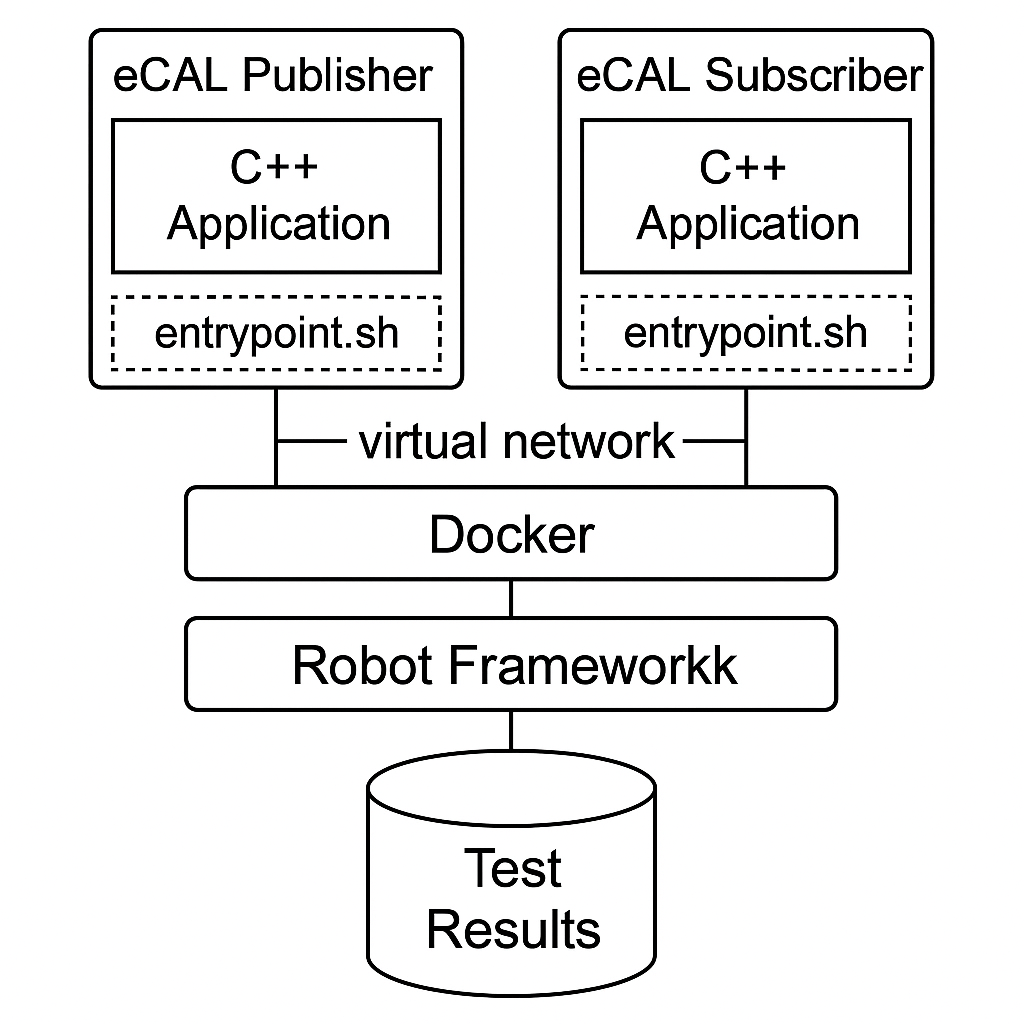
\includegraphics[width=0.72\textwidth]{Images/test_architecture_diagram.png}
 	\caption{Overview of the test environment architecture}
 	\label{fig:test_architecture_diagram}
 \end{figure}
 
The core components of the test architecture are:

\begin{itemize}
	\item \textbf{eCAL Publisher and Subscriber}: Each eCAL node is built as a separate C++ application and runs in its own Docker container. These processes communicate via eCAL using shared topics.
	\item \textbf{Docker Network}: All containers are connected to a common virtual Docker network (e.g., \texttt{ecal\_test\_net}), which enables communication using the selected transport layers.
	\item \textbf{Robot Framework}: The test logic is defined using Robot Framework. It is responsible for starting containers, injecting faults, checking logs, and validating test success criteria.
	\item \textbf{Entrypoint Scripts}: Each container uses an \texttt{entrypoint.sh} script that decides which executable to run (e.g., a publisher, subscriber, or test orchestrator), based on input arguments.
	\item \textbf{eCAL Configuration Files}: Runtime behavior such as communication mode (e.g., UDP vs. SHM) is controlled using \texttt{ecal.yaml} files or configuration overrides in code.
\end{itemize}

The test environment supports all major eCAL communication modes:

\begin{itemize}
	\item \texttt{local\_shm}: Local communication using shared memory.
	\item \texttt{local\_udp}: Local communication using UDP multicast.
	\item \texttt{local\_tcp}: Local communication using TCP.
	\item \texttt{network\_udp}: Network communication using UDP multicast.
	\item \texttt{network\_tcp}: Network communication using TCP.\\
\end{itemize}

This flexible design allows for testing a wide range of scenarios, including those where communication modes must be explicitly selected or changed during runtime. The environment also allows easy simulation of errors, such as killing a process, disconnecting a network, or injecting delays, which are critical for the validation of robustness.

\subsection{Implementation of the Test Infrastructure}

The integration test infrastructure for eCAL was designed to be modular, reusable, and easy to extend. It allows new test cases to be added or removed quickly by following a consistent folder structure and execution pattern. This is particularly useful for one of the most common use cases in test-driven development: adding a new test scenario with minimal overhead.

\vspace{0.5em}
Each component of the infrastructure follows a clear responsibility, which improves maintainability and simplifies debugging. The separation of test logic (e.g., message exchange and failure simulation) and infrastructure logic (e.g., container orchestration) ensures clean design and scalability.

\vspace{1em}
\textbf{1. MyDockerLibrary.py}

\vspace{0.3em}
This custom Python library for Robot Framework provides keywords to manage Docker containers. It offers reusable functions for starting and stopping containers, retrieving logs, checking exit codes, and simulating network disconnections. It abstracts low-level Docker interactions into simple, test-ready keywords.

\vspace{0.5em}
A typical use case is stopping and cleaning up test containers after execution. Listing~\ref{lst:docker_py_stop} shows a simplified implementation of the \texttt{Stop Container} keyword in Python, which handles safe shutdown and removal. Listing~\ref{lst:docker_robot_stop} illustrates how the keyword is used in a Robot Framework test case.

\begin{lstlisting}[style=cppstyle, language=Python, caption={Example keyword implementation in \texttt{MyDockerLibrary.py}}, label={lst:docker_py_stop}, captionpos=b]
 @keyword
  def stop_container(self, name):
    if name in self.containers:
       try:
           self.containers[name].stop()
           self.containers[name].remove()
       except NotFound:
           BuiltIn().log_to_console(f"Container {name} 
           already removed.")
       finally:
           self.containers.pop(name, None)
\end{lstlisting}

\begin{lstlisting}[style=cppstyle, caption={Calling \texttt{Stop Container} in a Robot Framework test}, label={lst:docker_robot_stop}, captionpos=b]
*** Settings ***
 Library           lib/MyDockerLibrary.py	

*** Test Cases ***
 Start Test
  Start Container    my_test_container
  
 ---Test Implementation here---  
 
 Cleanup After Test
  Stop Container    my_test_container
\end{lstlisting}


\vspace{1em}
\textbf{2. GlobalPathsLibrary.py}

\vspace{0.3em}
This library handles dynamic path and tag resolution across all test modules. It defines the active test case, provides access to configuration scripts, and ensures that Docker image names, container labels, and result folders are consistently named and resolved.

\vspace{1em}
\textbf{3. ecal\_config\_helper.h / .cpp}

\vspace{0.3em}
This shared C++ utility is responsible for configuring communication parameters such as transport mode and layer activation. It includes two central helper functions:

\begin{itemize}
	\item \texttt{wait\_for\_subscriber()} – ensures that messages are only published once a subscriber is available (see Listing~\ref{lst:wait_for_subscriber}).
	\item \texttt{setup\_ecal\_configuration()} – configures the desired communication mode (e.g., UDP, TCP, SHM) for each process (see Listing~\ref{lst:setup_ecal}).
\end{itemize}

\begin{lstlisting}[style=cppstyle, caption={Simplified wait\_for\_subscriber logic}, label={lst:wait_for_subscriber}, captionpos=b]
 void wait_for_subscriber(std::string topic){
   while (!has_subscriber(topic)){
     sleep_for(std::chrono::milliseconds(100));
  }
 }
\end{lstlisting}

\begin{lstlisting}[style=cppstyle, caption={Partial example for UDP setup}, label={lst:setup_ecal}, captionpos=b]
 if (mode == "local_udp"){
  config.communication_mode = 
                      eCAL::eCommunicationMode::local;
   if (is_publisher){
      config.publisher.layer_priority_local = 
                       {eCAL::TransportLayer::udp_mc};
   } else {
       config.subscriber.layer.shm.enable = false;
       config.subscriber.layer.udp.enable = true;
       config.subscriber.layer.tcp.enable = false;
    }
  }
\end{lstlisting}

\vspace{1em}
\textbf{5. build\_images.sh}

\vspace{0.3em}
This shell script builds the Docker images required for each test. It invokes CMake to compile the C++ test binaries and packages them together with all dependencies. This ensures consistency between test environments and local development.

\vspace{1em}
\textbf{4. entrypoint.sh}

\vspace{0.3em}
This is the entry script executed inside each container. It uses the given arguments (e.g., role: publisher or subscriber) to launch the correct binary with matching configuration. It also supports scenarios where both publisher and subscriber or multiple binarys are launched together inside the same container.

\vspace{1em}
The infrastructure enables consistent and isolated execution across all test cases while remaining flexible enough to simulate failures, delays, or disconnects. New modes or roles can be added without modifying the core infrastructure.

\subsection{Test Case Design}

This section presents selected integration test cases that were implemented to validate the core behaviors of the eCAL middleware. The tests are executed using Robot Framework and Docker-based containers and make use of the infrastructure described in Section~5.2. Each test focuses on a specific aspect of publisher-subscriber communication and follows a consistent structure.

\vspace{1em}
For every test case, the objective, execution steps, and success criteria are described. In addition, code examples are provided to illustrate important implementation details, such as how publishers and subscribers are configured and how messages are processed. Each test case ends with a short evaluation, which reflects on the observed behavior and explains how the results contribute to the overall test strategy.

\vspace{1em}
\subsubsection*{Test Case 1: Basic Publisher to Subscriber Communication}

\textbf{Objective:}

\vspace{0.4em}
Ensure that a message published by a single publisher is reliably received by a single subscriber using a specific transport layer (e.g., shared memory, TCP or UDP) (see Table~\ref{tab:basic_comm_test}).

\vspace{0.5em}
\textbf{Execution:}
\begin{itemize}
	\item In local modes (e.g., \texttt{local shm}, \texttt{local udp}), the publisher and subscriber run inside a single container.
	\item In network modes (e.g., \texttt{network udp}, \texttt{network tcp}), the publisher and subscriber run in separate containers connected via a Docker network.
	\item The publisher sends a small binary payload of value \texttt{42} (repeated) and logs each send event.
	\item The subscriber listens on the topic, logs received values, and exits successfully if the expected messages where received within the timeout window.
\end{itemize}

\textbf{Success Criteria:}
\begin{itemize}
	\item Subscriber receives 100\,\% of all messages sent.
	\item No crashes or communication timeouts occur.
	\item The subscriber exits with return code \texttt{0}.
\end{itemize}

\begin{table}[H]
	\centering
	\begin{tabular}{@{}llll@{}}
		\toprule
		\textbf{Component} & \textbf{Role} & \textbf{Transport Mode} & \textbf{Payload} \\
		\midrule
		basic\_pub  & Publisher  & All Modes  & \texttt{0x2A} (42) \\
		basic\_sub  & Subscriber & All Modes  & 42 \\
		\bottomrule
	\end{tabular}
	\caption{Configuration for Basic Communication Test}
	\captionsetup{position=bottom}
	\label{tab:basic_comm_test}
\end{table}


\textbf{Code Examples:}

\vspace{0.4em}
To illustrate key aspects of the basic communication test, the following code excerpts highlight how the publisher and subscriber are implemented.

\vspace{1em}
The publisher creates a binary buffer of size 10 where each byte is set to \texttt{0x2A} (decimal 42). This value is used consistently across all test scenarios to simplify result verification (see Listing \ref{lst:basic_pub_send}).

\vspace{1em}
The subscriber callback reads the first byte of the received buffer and casts it to an integer. This ensures that the payload can be easily validated (see Listing \ref{lst:basic_sub_receive}).
\vspace{0.5em}

\begin{lstlisting}[style=cppstyle, caption={Binary buffer with value 42 used by the publisher}, label={lst:basic_pub_send}, captionpos=b]
	std::vector<unsigned char> buffer(10, 42);
	pub.Send(buffer.data(), buffer.size());
\end{lstlisting}

\begin{lstlisting}[style=cppstyle, caption={Extracting first byte from the received message in subscriber}, label={lst:basic_sub_receive}, captionpos=b]
	int value = static_cast<int>(
	static_cast<const unsigned char*>(data_.buffer)[0]
	);
\end{lstlisting}

\begin{lstlisting}[style=cppstyle, caption={Argument setup using TCLAP in both publisher and subscriber}, label={lst:tclap_basic}, captionpos=b]
 TCLAP::ValueArg<std::string> mode_arg(
 "m", "mode", "Transport mode", true, "", "string");
 
 TCLAP::ValueArg<std::string> topic_arg(
 "t", "topic", "Topic name", false, "test_topic", "string");
 
 TCLAP::ValueArg<std::string> name_arg(
 "n", "name", "eCAL node name", false, "pub_test", "string");
 
 TCLAP::ValueArg<int> count_arg(
 "c", "count", "Number of messages", false, 3, "int");
 
 TCLAP::ValueArg<int> delay_arg(
 "d", "delay", "Delay between sends", false, 1000, "int");
\end{lstlisting}

\vspace{0.4em}
The configuration with TLCAP in Listing \ref{lst:tclap_basic} allows full flexibility for running the same binary with different roles and transport modes. The \texttt{--mode} parameter (e.g., \texttt{local\_tcp}) enables switching between eCAL transport layers without modifying the code. The use of TCP is especially useful for tests that simulate network scenarios across Docker containers, where shared memory is not apply able.

\vspace{1em}

\textbf{Evaluation:}

\vspace{0.4em}
This basic test confirms that eCAL reliably delivers messages across all supported transport modes under ideal conditions. The results show that communication remains consistent in both local and networked setups, provided the configuration parameters are correctly applied. This test serves as the foundation for more advanced scenarios such as crash handling, message validation, or multi-topic communication.


\vspace{1em}
\vspace{1em}
\subsubsection*{Test Case 2: Multiple Publishers and Multiple Subscribers on One Topic}

\textbf{Objective:}

\vspace{0.4em}
Verify that multiple publishers can send distinct payloads on the same topic and that multiple subscribers can receive both streams reliably.

\vspace{0.5em}
\textbf{Execution:}
\begin{itemize}
	\item Two publishers send different payloads (42 and 43) on the same topic.
	\item Two subscribers listen to the same topic and count how many messages they receive for each value.
	\item All four nodes run either in a single container (local mode) or separate containers connected via Docker network (network mode).
\end{itemize}

\textbf{Success Criteria:}
\begin{itemize}
	\item Each subscriber receives 100\,\% of the messages from both publishers.
	\item No crash or message loss occurs during transmission.
	\item All containers exit with return code \texttt{0}.
\end{itemize}

\begin{table}[H]
	\centering
	\begin{tabular}{@{}llll@{}}
		\toprule
		\textbf{Component}     & \textbf{Role}    & \textbf{Transport Mode} & \textbf{Payload} \\
		\midrule
		multi\_publisher       & Publisher        & All Modes               & \texttt{0x2B} (43) \\
		multi\_publisher2      & Publisher        & All Modes               & \texttt{0x2A} (42) \\
		multi\_subscriber      & Subscriber       & All Modes               & Both              \\
		multi\_subscriber2     & Subscriber       & All Modes               & Both              \\
		\bottomrule
	\end{tabular}
	\caption{Configuration for Multi-Publisher and Multi-Subscriber Test}
	\label{tab:multi_pub_sub_test}
\end{table}

\textbf{Code Examples:}
\vspace{0.4em}

Listing~\ref{lst:multi_pub1_send} shows how \texttt{multi\_publisher} sends a binary payload containing value 43. Listing~\ref{lst:multi_pub2_send} illustrates the second publisher, which uses value 42. Both publishers send 15 messages with a 1000\,ms delay between sends.
\vspace{0.5em}
\begin{lstlisting}[style=cppstyle, caption={Publisher 1 sends 0x2B (43)}, label={lst:multi_pub1_send}, captionpos=b]
 std::vector<unsigned char> buffer(10, 43);
 pub.Send(buffer.data(), buffer.size());
\end{lstlisting}
\vspace{0.5em}
\begin{lstlisting}[style=cppstyle, caption={Publisher 2 sends 0x2A (42)}, label={lst:multi_pub2_send}, captionpos=b]
 std::vector<unsigned char> buffer(10, 42);
 pub.Send(buffer.data(), buffer.size());
\end{lstlisting}

Each subscriber uses a callback function that increments counters depending on the first byte received. The values 42 and 43 are tracked separately (see Listing~\ref{lst:multi_sub_receive}).
\vspace{0.5em}
\begin{lstlisting}[style=cppstyle, caption={Subscriber callback counting 42 and 43}, label={lst:multi_sub_receive}, captionpos=b]
 if (value == 42) ++count_42;
 if (value == 43) ++count_43;
\end{lstlisting}

\vspace{0.5em}
\textbf{Evaluation:}

\vspace{0.4em}
This test confirms that eCAL supports N:N communication over a shared topic. Both subscribers successfully received messages from both publishers in all tested transport modes. This demonstrates the middleware's ability to handle concurrent sources and destinations. This is a critical feature for scenarios involving aggregation, monitoring, or distributed decision-making.

\vspace{1em}
From a combinatorial perspective, a complete evaluation of the publish-subscribe model would require testing all communication patterns: one-to-one (1:1), one-to-many (1:N), many-to-one (N:1), and many-to-many (N:N). In practice, however, N:N scenarios inherently cover the functional aspects of both 1:N and N:1 communication patterns. This is because every N:N test includes multiple publishers and subscribers and therefore implicitly verifies the correctness of message delivery from one to many (1:N) and from many to one (N:1) within the same execution.

\vspace{1em}
By implementing N:N tests across all five eCAL transport modes (\texttt{local\_shm}, \texttt{local\_udp}, \texttt{local\_tcp}, \texttt{network\_udp}, \texttt{network\_tcp}), we effectively validate the core functionality and robustness of the middleware under realistic and complex conditions. This strategic reduction in test permutations allows for efficient validation without sacrificing coverage.

\vspace{1em}
\vspace{1em}
\subsubsection*{Test Case 3: Publisher Crash During Transmission}

\textbf{Objective:} 

\vspace{0.4em}
Evaluate the system's resilience when one publisher crashes mid-transmission, and ensure that the subscriber still receives messages from the remaining active publisher.

\vspace{0.5em}
\textbf{Execution:}
\begin{itemize}
	\item Two publishers are started: one sends \texttt{42} and crashes after 10 messages, the other sends \texttt{43} continuously.
	\item One subscriber is launched to receive messages from both.
	\item The test runs in all communication modes (local and network).
	\item The subscriber counts messages from both publishers and exits after a fixed timeout.
\end{itemize}

\textbf{Success Criteria:}
\begin{itemize}
	\item The subscriber receives at least 25 messages with value \texttt{43}.
	\item The number of \texttt{42} messages is below the crash threshold (between 5 and 11).
	\item The subscriber exits with return code \texttt{0}.
\end{itemize}

\begin{table}[H]
	\centering
	\begin{tabular}{@{}llll@{}}
		\toprule
		\textbf{Component} & \textbf{Role}     & \textbf{Transport Mode} & \textbf{Payload} \\
		\midrule
		crash\_pub         & Publisher         & All Modes               & \texttt{0x2A} (42) \\
		test\_pub          & Publisher         & All Modes               & \texttt{0x2B} (43) \\
		test\_sub          & Subscriber        & All Modes               & 42 + 43 \\
		\bottomrule
	\end{tabular}
	\caption{Configuration for Crash Resilience Test}
	\label{tab:crash_resilience}
\end{table}

\vspace{0.5em}

\textbf{Code Examples:}

\vspace{0.4em}
The crashing publisher sends a few messages and then exits by calling \texttt{std::abort()}, simulating a runtime failure (Listing~\ref{lst:crash_pub_send}). Meanwhile, the test publisher continues normal operation (Listing~\ref{lst:test_pub_send}).

\vspace{0.5em}
\begin{lstlisting}[style=cppstyle, caption={Crash publisher sends and exits after 10 messages}, label={lst:crash_pub_send}, captionpos=b]
 for (int i = 0; i < total_arg.getValue(); ++i){
  pub.Send(buf.data(), buf.size());
  sleep_for(delay_ms);
  if (i == crash_at_arg.getValue()){
   std::abort();  // Simulate crash
  }
 }
\end{lstlisting}
\vspace{0.5em}
\begin{lstlisting}[style=cppstyle, caption={Resilient publisher continues sending messages}, label={lst:test_pub_send}, captionpos=b]
 for (int i = 0; i < count && eCAL::Ok(); ++i){
  pub.Send(buffer.data(), buffer.size());
  sleep_for(delay_ms);
 }
\end{lstlisting}

The subscriber counts received values and returns 0 only if enough \texttt{43} values are seen and no unexpected continuation from the crashed publisher occurs (Listing~\ref{lst:crash_sub_eval}).

\vspace{0.5em}
\begin{lstlisting}[style=cppstyle, caption={Subscriber decision logic}, label={lst:crash_sub_eval}, captionpos=b]
 if (count_43 >= 25 && count_42 < 11 && count_42 > 4){
   return 0; // Success: resilient communication
 }else{
   return 1; // Failure: not enough or unexpected data
 }
\end{lstlisting}

\vspace{0.5em}

\newpage
\textbf{Evaluation:}

This test demonstrates that eCAL remains fully functional and continues to deliver messages even when one of the publishers crashes unexpectedly. The second publisher, which sends payload \texttt{43}, continues to operate without interruption. This confirms that the failure of one communication node does not affect the functionality of others. The test was executed in all supported eCAL transport modes, showing that this reliability is consistent regardless of the communication layer.

\vspace{1em}

The use of a crash publisher simulates real-world process failures, and the test verifies that message delivery remains uninterrupted. By comparing the message counts, the system ensures that no "phantom" messages are received after the crash point. This approach can be used as a template for testing fault tolerance in distributed IPC systems.

\vspace{1em}
\subsubsection*{Test Case 4: Subscriber Crash During Reception}

\textbf{Objective:} \\
Verify that the communication remains stable even when one subscriber crashes while receiving large messages.

\vspace{0.5em}
\textbf{Execution:}
\begin{itemize}
	\item A \texttt{large\_publisher} sends three large messages (each about 50\,MB) on the same topic.
	\item One \texttt{crash\_subscriber} is configured to crash after a short time during message reception.
	\item One \texttt{test\_subscriber} continues running and should receive all messages correctly.
	\item The test is executed in all supported eCAL transport modes, except for local UDP which cannot handle large messages.
	\item A special variant uses SHM with \texttt{zero\_copy\_mode = true} to verify robustness of shared memory access.
\end{itemize}

\textbf{Success Criteria:}
\begin{itemize}
	\item The stable subscriber exits with return code \texttt{0} and logs successful message reception.
	\item The crashing subscriber terminates due to a simulated failure after a few seconds.
	\item The publisher completes message delivery without interruption or failure.
	\item In SHM mode with Zero-Copy, shared memory corruption or deadlocks must not occur.
\end{itemize}

\begin{table}[H]
	\centering
	\begin{tabular}{@{}llll@{}}
		\toprule
		\textbf{Component} & \textbf{Role}       & \textbf{Transport Mode} & \textbf{Payload} \\
		\midrule
		large\_publisher   & Publisher           & All Modes               & $\sim$50\,MB     \\
		crash\_subscriber  & Subscriber (crash)  & All Modes               & $\sim$50\,MB     \\
		test\_subscriber   & Subscriber (stable) & All Modes               & $\sim$50\,MB     \\
		\bottomrule
	\end{tabular}
	\caption{Configuration for Crash During Reception Test}
	\label{tab:sub_crash_receive}
\end{table}

\vspace{0.5em}
\textbf{Code Example:}

The crashing subscriber aborts its process intentionally after two seconds of runtime if it receives any message (see Listing~\ref{lst:sub_crash_logic}).

\begin{lstlisting}[style=cppstyle, caption={Crash condition inside subscriber receive callback}, label={lst:sub_crash_logic}, captionpos=b]
 void OnReceive(
    const eCAL::STopicId&, const eCAL::SDataTypeInformation&,
    const eCAL::SReceiveCallbackData& data_)
 {
  std::cout << "[Crash_Sub] Received " 
  << data_.buffer_size << " bytes\n";
    		
  if (elapsedtime >= 2) {
   std::cerr << "[Crash_Sub] Simulating crash after 2 sec";
   std::abort();
  }
 }

\end{lstlisting}

To simulate high-throughput conditions, the publisher sends three 50\,MB messages and logs each transmission result (see Listing~\ref{lst:large_pub_send}).

\begin{lstlisting}[style=cppstyle, caption={Large message publisher with send confirmation}, label={lst:large_pub_send}, captionpos=b]
 std::string buffer(50L * 1024L * 1024L, 'X');
 for (int i = 0; i < count; ++i){
   bool sent = pub.Send(buffer.data(), buffer.size());
   std::cout << "[Publisher] Send result: " 
             << (sent ? "pass" : "fail");
 }
\end{lstlisting}

\vspace{0.5em}

\newpage
\textbf{Evaluation:}

\vspace{0.4em}
This test confirms that eCAL maintains stable communication even when a subscriber crashes during the reception of a large message. In all tested configurations except the Zero-Copy SHM variant, the system behaved as expected: the publisher completed its transmission successfully, and the stable subscriber received all messages without interruption. The crash was isolated to the failing subscriber, indicating proper error containment and robustness of the communication layer.

\vspace{1em}
The variant using Zero-Copy in Shared Memory mode highlighted a specific weakness in fault isolation. In Zero-Copy mode, the publisher shares direct memory access with subscribers, which eliminates the need for memory copying and significantly improves performance in high-throughput scenarios. However, this optimization also introduces a stronger coupling between processes at the memory level.

\vspace{1em}
If a subscriber crashes while holding a pointer to shared memory, the publisher (or other subscribers) may experience access violations, resource locks, or inconsistent memory states. This was observed during the test: although the publisher attempted to continue sending data, the shared memory segment could no longer be accessed safely once the crashing subscriber aborted during callback execution. 

\vspace{1em}
Therefore, while Zero-Copy SHM offers performance advantages, it requires careful handling in fault-tolerant systems. Mechanisms such as memory fencing, process monitoring, or fallback copy modes should be considered if system resilience is a priority.

\vspace{1em}
In conclusion, this test underscores both the reliability of eCAL in standard SHM, TCP, and UDP scenarios and the current limitations when using Zero-Copy SHM without additional safeguards. Future testing or deployment scenarios should carefully consider the trade-off between performance and fault tolerance when using advanced features like Zero-Copy.

\newpage

\vspace{1em}
\subsubsection*{Test Case 5: Network Failure Simulation}

TODO

\newpage
\subsection{Handling of Edge Cases}

In addition to testing typical communication flows, the test infrastructure also covers a variety of edge cases that may occur in distributed systems. These cases are particularly important for evaluating the robustness and fault tolerance of the eCAL middleware under non-ideal conditions.

\vspace{0.5em}
The following categories of edge cases are addressed:

\begin{itemize}
	\item \textbf{Timing jitter and delays} \\
	To simulate unstable timing behavior, artificial delays are introduced using \texttt{sleep} call to manipulate network latency. This helps verify whether eCAL nodes can still synchronize and communicate reliably under varying timing conditions.
	
	\item \textbf{Crash simulation} \\
	Component failures are simulated by forcefully stopping or disconnecting Docker containers. This reflects real-world scenarios such as sudden application crashes or network cable unplugging. The system’s ability to recover, reconnect, or log the error is then observed.
	
	\item \textbf{Missing communication partners} \\
	In some tests, publishers are started without any active subscribers. This tests whether the publisher behaves correctly in absence of receivers, without blocking or generating errors.
\end{itemize}

\vspace{0.5em}
To evaluate the outcome of these tests, different observation methods are applied:

\begin{itemize}
	\item \textbf{Exit code monitoring} \\
	Each container returns an exit code upon completion. A code of \texttt{0} indicates successful execution, while non-zero values signal unexpected behavior or test failure.
	
	\item \textbf{Log analysis} \\
	Container logs are collected and printed by the Robot Framework. These logs include important debug messages and warnings generated by the eCAL nodes and the test logic.
	
	\item \textbf{Payload validation} \\
	In several tests, the payload value is checked directly to verify that messages were received correctly and from the expected source.
\end{itemize}

This structured approach to handling edge cases ensures that both functional correctness and system reliability are fully tested under the most challenging conditions.


\subsection{Automation and Repeatability}

One of the main goals of the integration test design is to ensure that all tests can be executed in a fully automated and repeatable way. Automation is essential for running regression tests frequently and reliably—especially when integrating the tests into CI/CD pipelines.

\vspace{0.9em}
The tests are executed using Robot Framework and can be triggered with a single command:

\begin{verbatim}
	robot --outputdir results network_crash.robot
\end{verbatim}

\vspace{0.5em}
This command runs the specified test and stores the output files in the \texttt{results} directory. The following artifacts are automatically generated after each run:

\begin{itemize}
	\item \textbf{log.html} – Detailed step-by-step execution log with console output
	\item \textbf{report.html} – Summary report with pass/fail statistics
	\item \textbf{output.xml} – Raw result data (used for machine-readable processing or CI systems)
\end{itemize}

\vspace{0.5em}
The simplicity and structure of this test approach makes it well suited for integration into CI/CD systems such as GitHub Actions or GitLab CI. These systems can be configured to run the test suite automatically after every commit or pull request, ensuring that communication functionality remains stable even during ongoing development.

\vspace{0.9em}
Furthermore, since Docker is used for test isolation, the tests are highly portable and can run in local development environments, on build servers, or in virtualized testing infrastructure with minimal setup.

\subsection{Summary}

The implementation of integration tests for eCAL showed that the combination of Docker and Robot Framework is well suited for testing inter-process communication in a modular and reproducible manner. The infrastructure allows test scenarios to be executed consistently and extended easily. Especially the ability to simulate component failures (e.g., network drop or process crash) proved to be helpful in analyzing system robustness.

\vspace{0.9em}
Basic communication patterns such as single or multiple publishers and subscribers worked reliably in all tested transport modes, including \texttt{local\_udp}, \texttt{local\_tcp}, and \texttt{network\_udp}. However, communication via \texttt{local\_shm} was not always functional in Docker containers due to the isolation between container namespaces, which limits shared memory usage. This restriction highlights an important consideration when testing IPC frameworks in containerized environments.

\vspace{0.9em}
The framework is already equipped to be extended with further test categories. For example, future work could include RPC-based communication, service availability tests, and metrics such as round-trip time or failure recovery time. Moreover, integration into CI/CD pipelines would enable automatic regression testing during development and deployment.

